\section{Vue 项目与模块}

这一章需要构建 Vue 项目(参考 1.4.2 节)。

\subsection{Vue 项目结构}

在创建完成后,一个标准的 webpack 文件(运用其他模板创建的项目也类似)结构如下:

\begin{figure}[H]
    \centering
    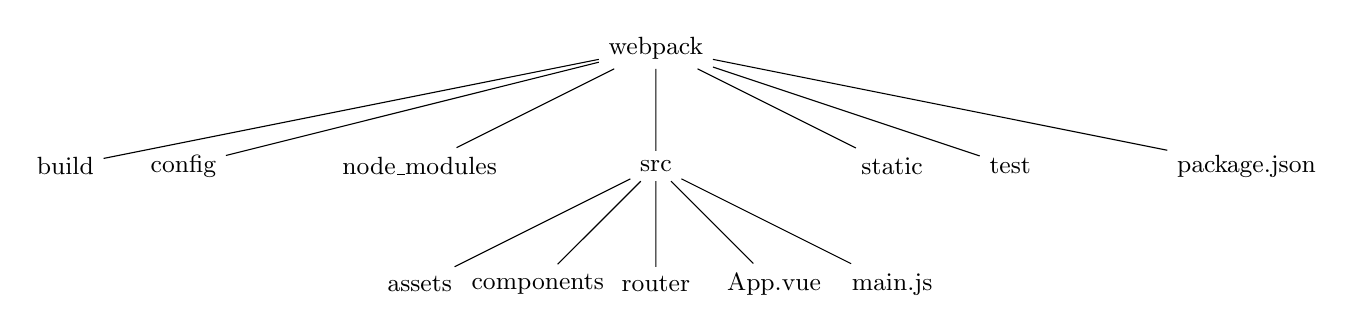
\begin{tikzpicture}[font=\small]
        \node {webpack} 
        child { node {build}}		
        child { node {config}}
        child [missing] {}	
        child { node {node\_modules}}
        child [missing] {}	
        child { node {src}
            child {node {assets}}
            child {node {components}}
            child {node {router}}
            child {node {App.vue}}
            child {node {main.js}}
        }	
        child [missing] {}	
        child { node {static}}	
        child { node {test}}	
        child [missing] {}	
        child { node {package.json}};
    \end{tikzpicture}
    \caption{webpack 文件结构}
    \label{fig:webpack 文件结构}
\end{figure}

其各个文件及文件夹用处如下表: